\chapter{v1: synthetic results and real-data failure}
\label{chap:v1results}
\label{chap:v1real}

This chapter is the v1 retrospective: how the three architectures
behaved when trained on the v1 dataset, both on the held-out synthetic
test segment (\cref{sec:v1-synth-results}) and on the four months of
real recordings (\cref{sec:v1-real-symptoms}). The takeaway --- the
system passes the synthetic benchmark very comfortably but fails on
real data --- is what motivates the rest of the report.

\section{Synthetic-test performance}
\label{sec:v1-synth-results}

\subsection{Training dynamics}

\Cref{fig:v1-training} overlays the train and validation losses and the
validation macro F1 of the three models.

\begin{figure}[H]
    \centering
    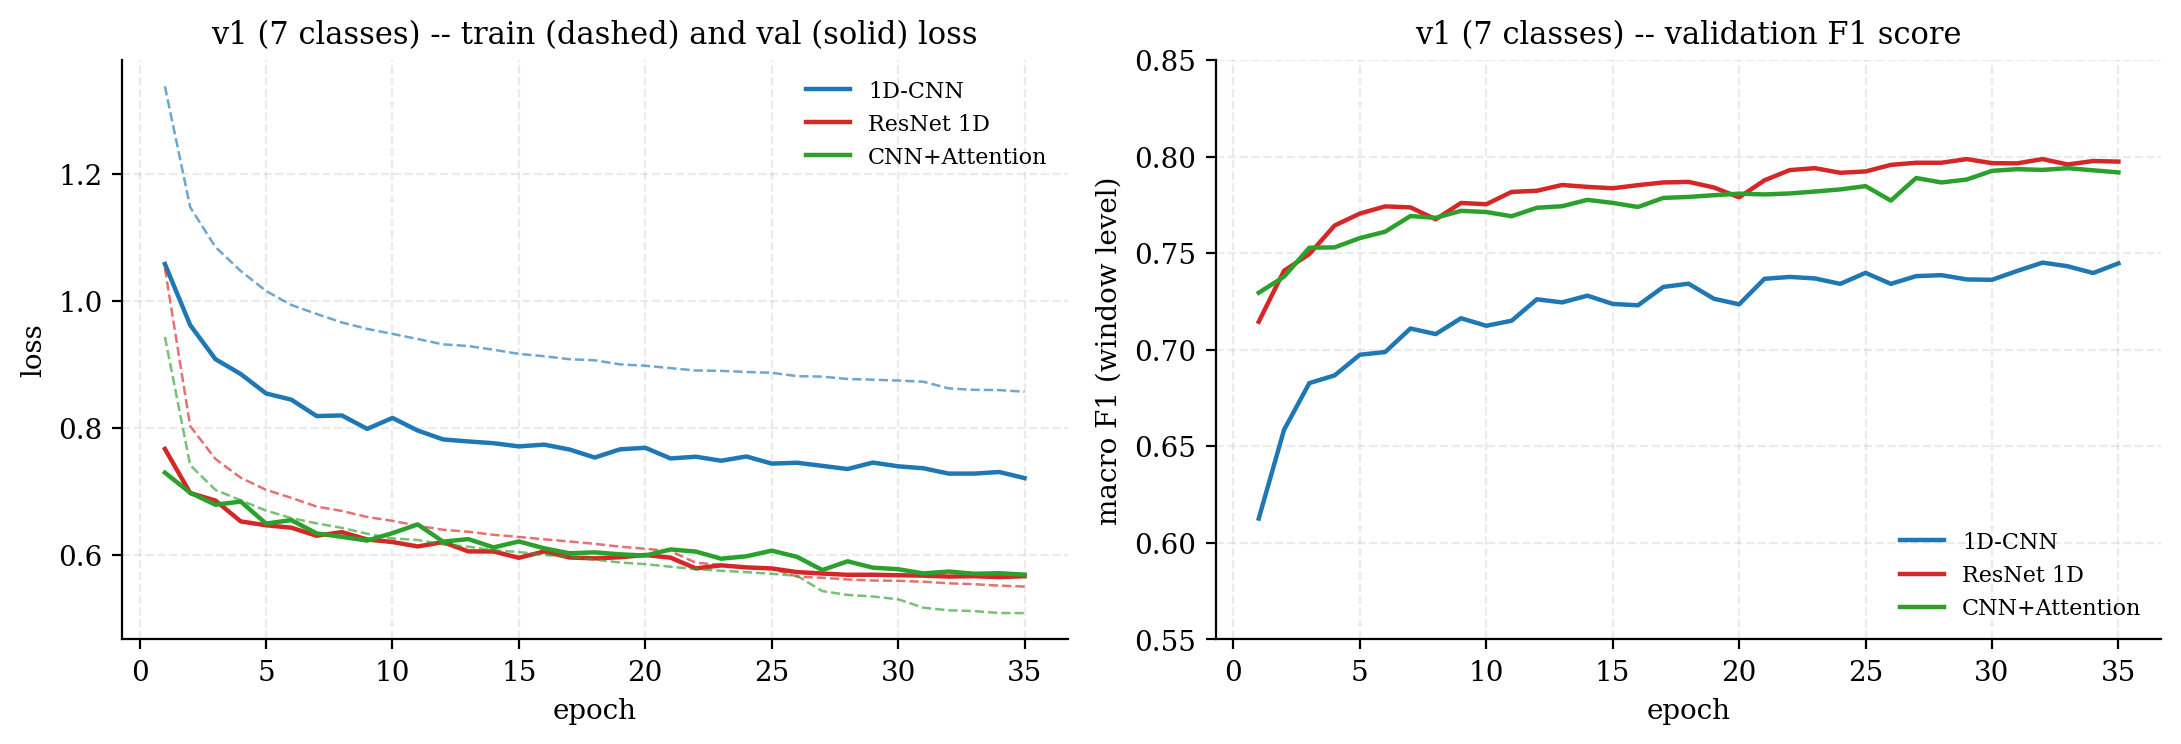
\includegraphics[width=\linewidth]{figures/v1_training_curves}
    \caption{v1 training dynamics. Left: train (dashed) and validation
    (solid) loss for the three models. Right: validation macro F1
    (window level). All three models converge within $35$ epochs and
    benefit from one or two learning-rate reductions.}
    \label{fig:v1-training}
\end{figure}

The residual network reaches a clearly lower validation-loss plateau
than the baseline 1D-CNN (about $0.57$ vs $0.72$), and so does the
attention model. Both more advanced models also start much higher on
the validation F1 axis already at the first epoch ($> 0.71$ versus
$0.61$ for the baseline).

\subsection{Event-level evaluation methodology}
\label{sec:event-eval}

For an operationally meaningful metric, we evaluate the system on a
continuous test segment using a \emph{detection-driven} protocol
implemented in \texttt{architectures/inference\_engine.py}.

A test segment of $100\,000$ samples (immediately following the
training portion) is fed to the network through a sliding window of
size $512$ and stride $10$; per-window probability outputs are averaged
into a per-sample probability trace $\hat{P} \in \R^{N \times K}$. A
sample is declared anomalous if $\hat{P}_{t, 0} < 0.3$; contiguous
anomalous regions form predicted events, with small gaps of up to
$50$ samples bridged. The class of a predicted event is the
\emph{argmax} of the cumulative probability vector across its samples.
True events are extracted from the ground-truth labels the same way;
a predicted event matches a true event whenever the two intervals
overlap, and the result is split into TPs, misclassifications, missed
events, and hallucinations. Per-class precision/recall/F1 are then
computed, and the report quotes the macro average across the anomaly
classes.

\subsection{v1 event-level results}

On the $100\,000$-sample v1 test segment, there are $59$ ground-truth
events. The event-level confusion matrices are shown in
\cref{fig:v1-confmat}.

\begin{figure}[H]
    \centering
    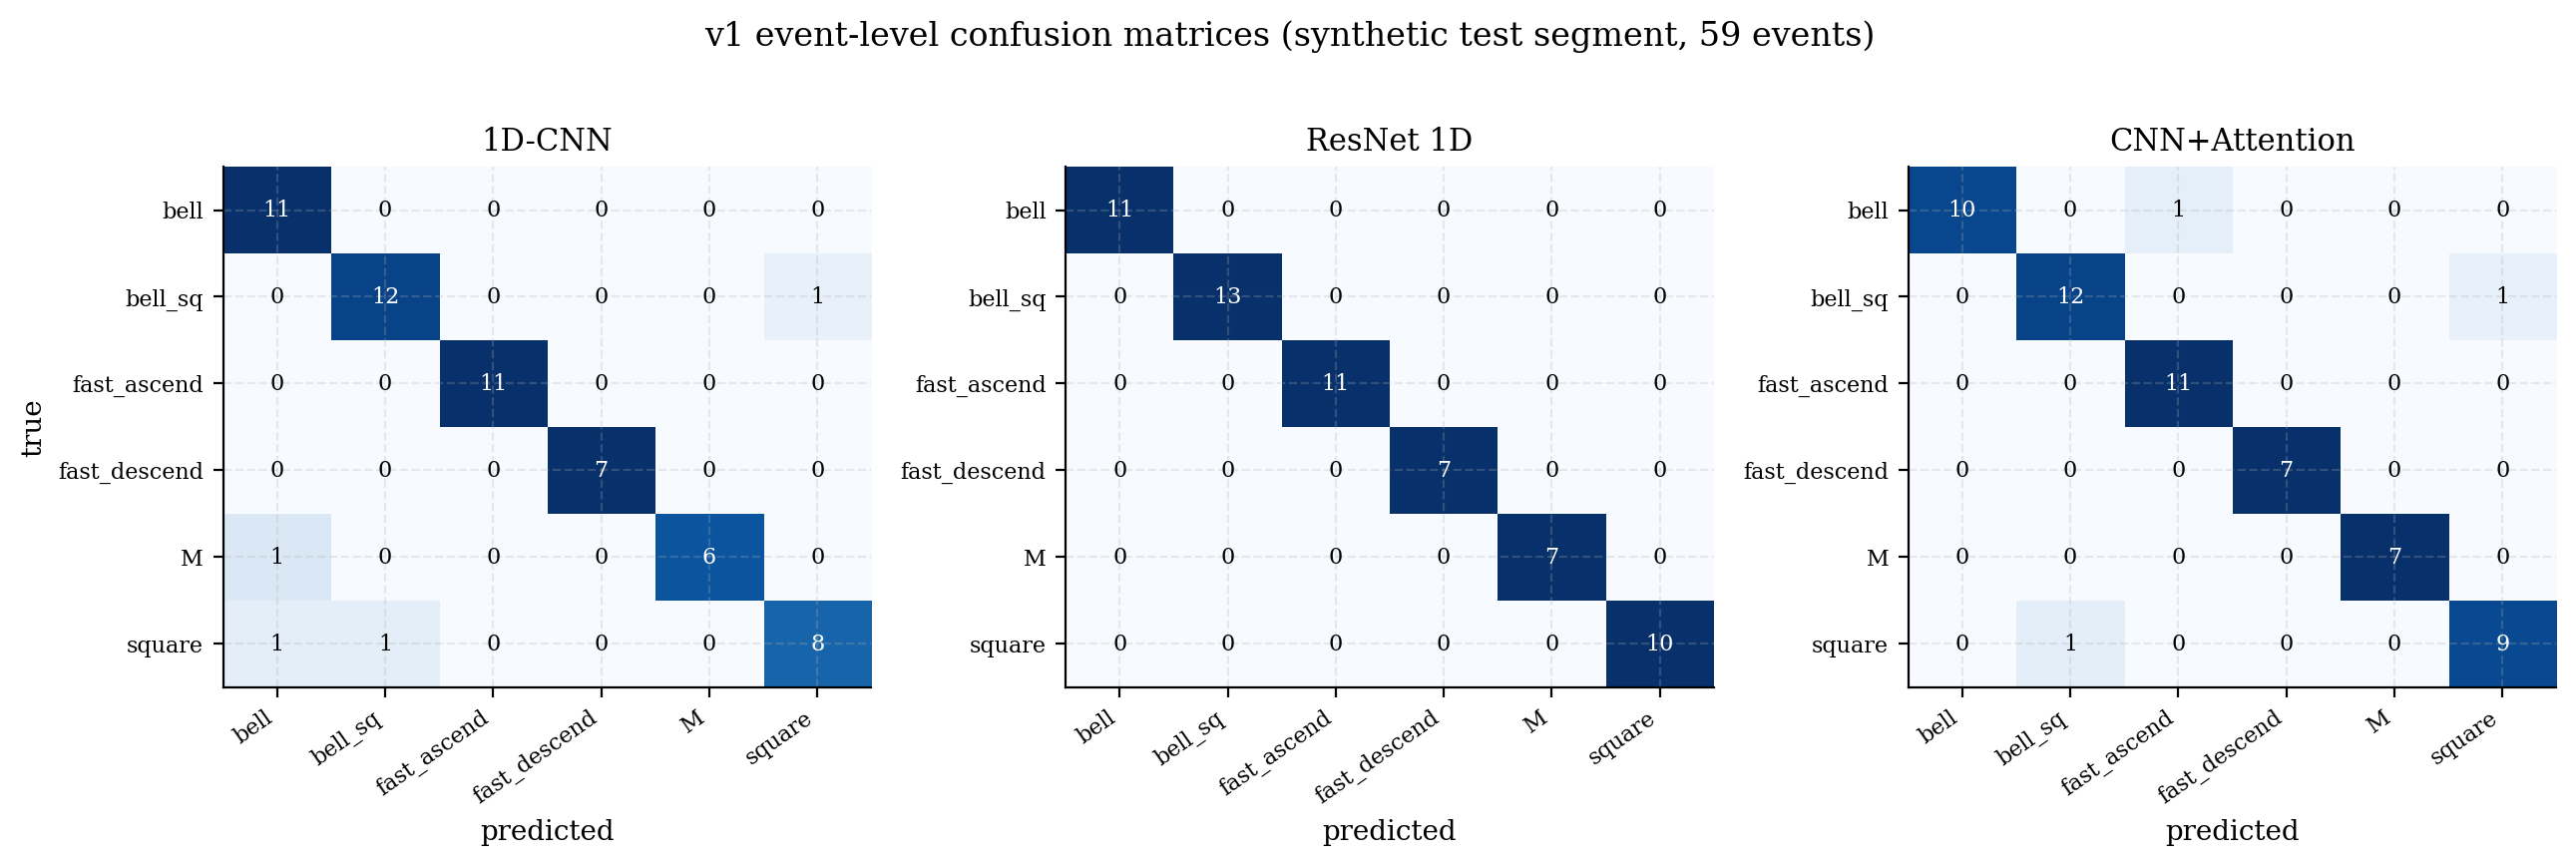
\includegraphics[width=\linewidth]{figures/v1_confusion_matrices}
    \caption{v1 event-level confusion matrices on the synthetic test
    segment. Cell colour is the row-normalised recall; the integer
    inside each cell is the raw event count. The residual network
    achieves a perfect classification; the attention model misses
    three events; the baseline 1D-CNN misses four events.}
    \label{fig:v1-confmat}
\end{figure}

The corresponding macro F1 scores are summarised in
\cref{tab:v1-event-f1}.

\begin{table}[H]
    \centering
    \footnotesize
    \begin{tabular}{lc}
        \toprule
        Model & Event-level macro F1 \\
        \midrule
        1D-CNN          & $0.934$ \\
        ResNet 1D       & $1.000$ \\
        CNN+Attention   & $0.955$ \\
        \bottomrule
    \end{tabular}
    \caption{v1 event-level macro F1 on the synthetic test segment
    (59 events). All three models cross the $90\%$ line; the residual
    network is flawless.}
    \label{tab:v1-event-f1}
\end{table}

A striking property of these results is that the false-positive rate
is essentially zero: predicted events that do not overlap any true
event are extremely rare on this segment. The trained system looks,
on its own training distribution, in very good shape.

\section{v1 robustness study}
\label{sec:v1-robustness}

To check whether the same hold under controlled stress, the robustness
script (\texttt{architectures/robustness\_test.py}) generates small
test datasets while sweeping two distortion parameters independently:
the background-noise standard deviation $\sigma$ (multiplied by
$m_{\text{noise}} \in [1, 3]$, with the anomaly amplitudes divided by
the same factor so the absolute SNR remains constant), and the
deformation-variance parameter $\nu$ (multiplied by $m_{\text{deform}}
\in [1, 8]$).

\begin{figure}[H]
    \centering
    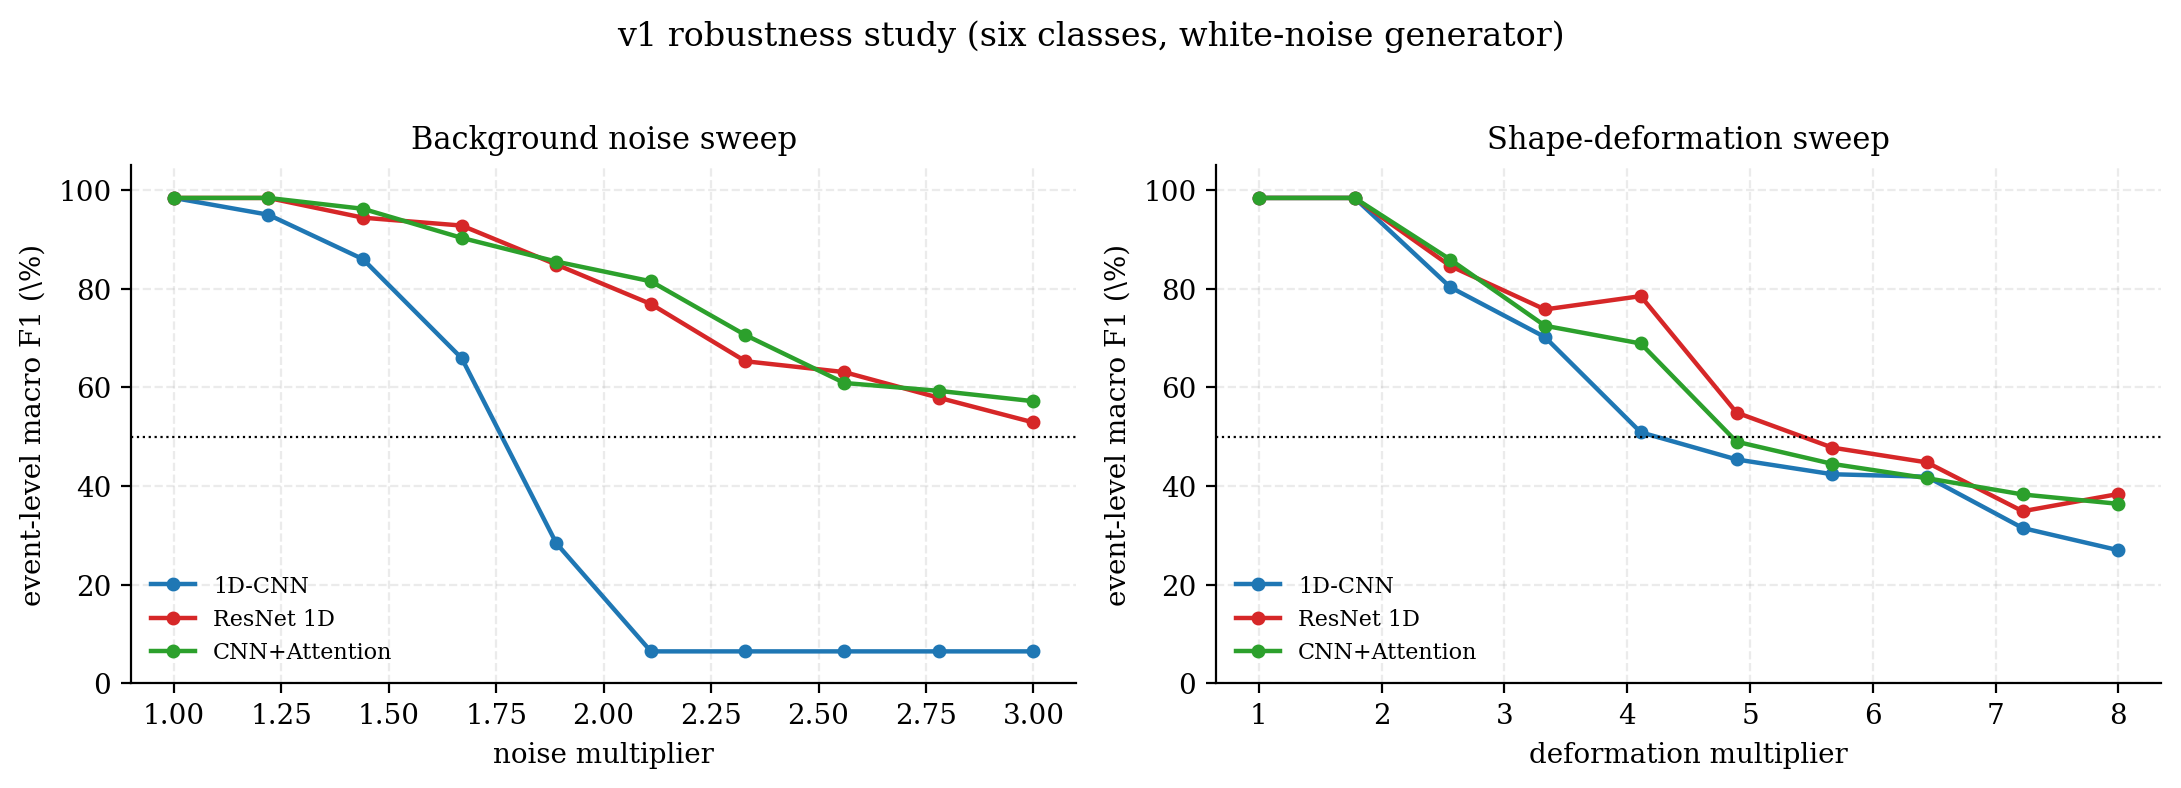
\includegraphics[width=\linewidth]{figures/v1_robustness}
    \caption{v1 robustness curves. Left: macro F1 vs. background-noise
    multiplier. Right: macro F1 vs. anomaly-shape deformation
    multiplier. The dotted line marks $50\%$ F1. The 1D-CNN drops
    sharply to a $\sim 7\%$ plateau under noise --- the hallmark of a
    classifier that has lost confidence in its features and collapses
    to a single class. The residual and attention models degrade much
    more gracefully.}
    \label{fig:v1-robustness}
\end{figure}

The two structural takeaways from \cref{fig:v1-robustness} are: (i)
residual connections + GroupNorm dramatically improve the noise
robustness of the network (the gap between the 1D-CNN and the ResNet
at $m_{\text{noise}} = 2$ is enormous); (ii) self-attention does not
buy any extra robustness on top of residual learning at $W = 512$,
because the window is too short for the attention mechanism to have
much extra context to exploit. The full discussion is identical to
what \cref{sec:rob-discuss} reports for v2.

\section{v1 on real data: three architecture-specific failures}
\label{sec:v1-real-symptoms}

The clean-test numbers above hide an alarming truth: when the same
trained v1 models are confronted with the real 2015 recordings, all
three behave poorly --- and each fails in its own way
(\cref{fig:v1-real-inference}).

\begin{figure}[H]
    \centering
    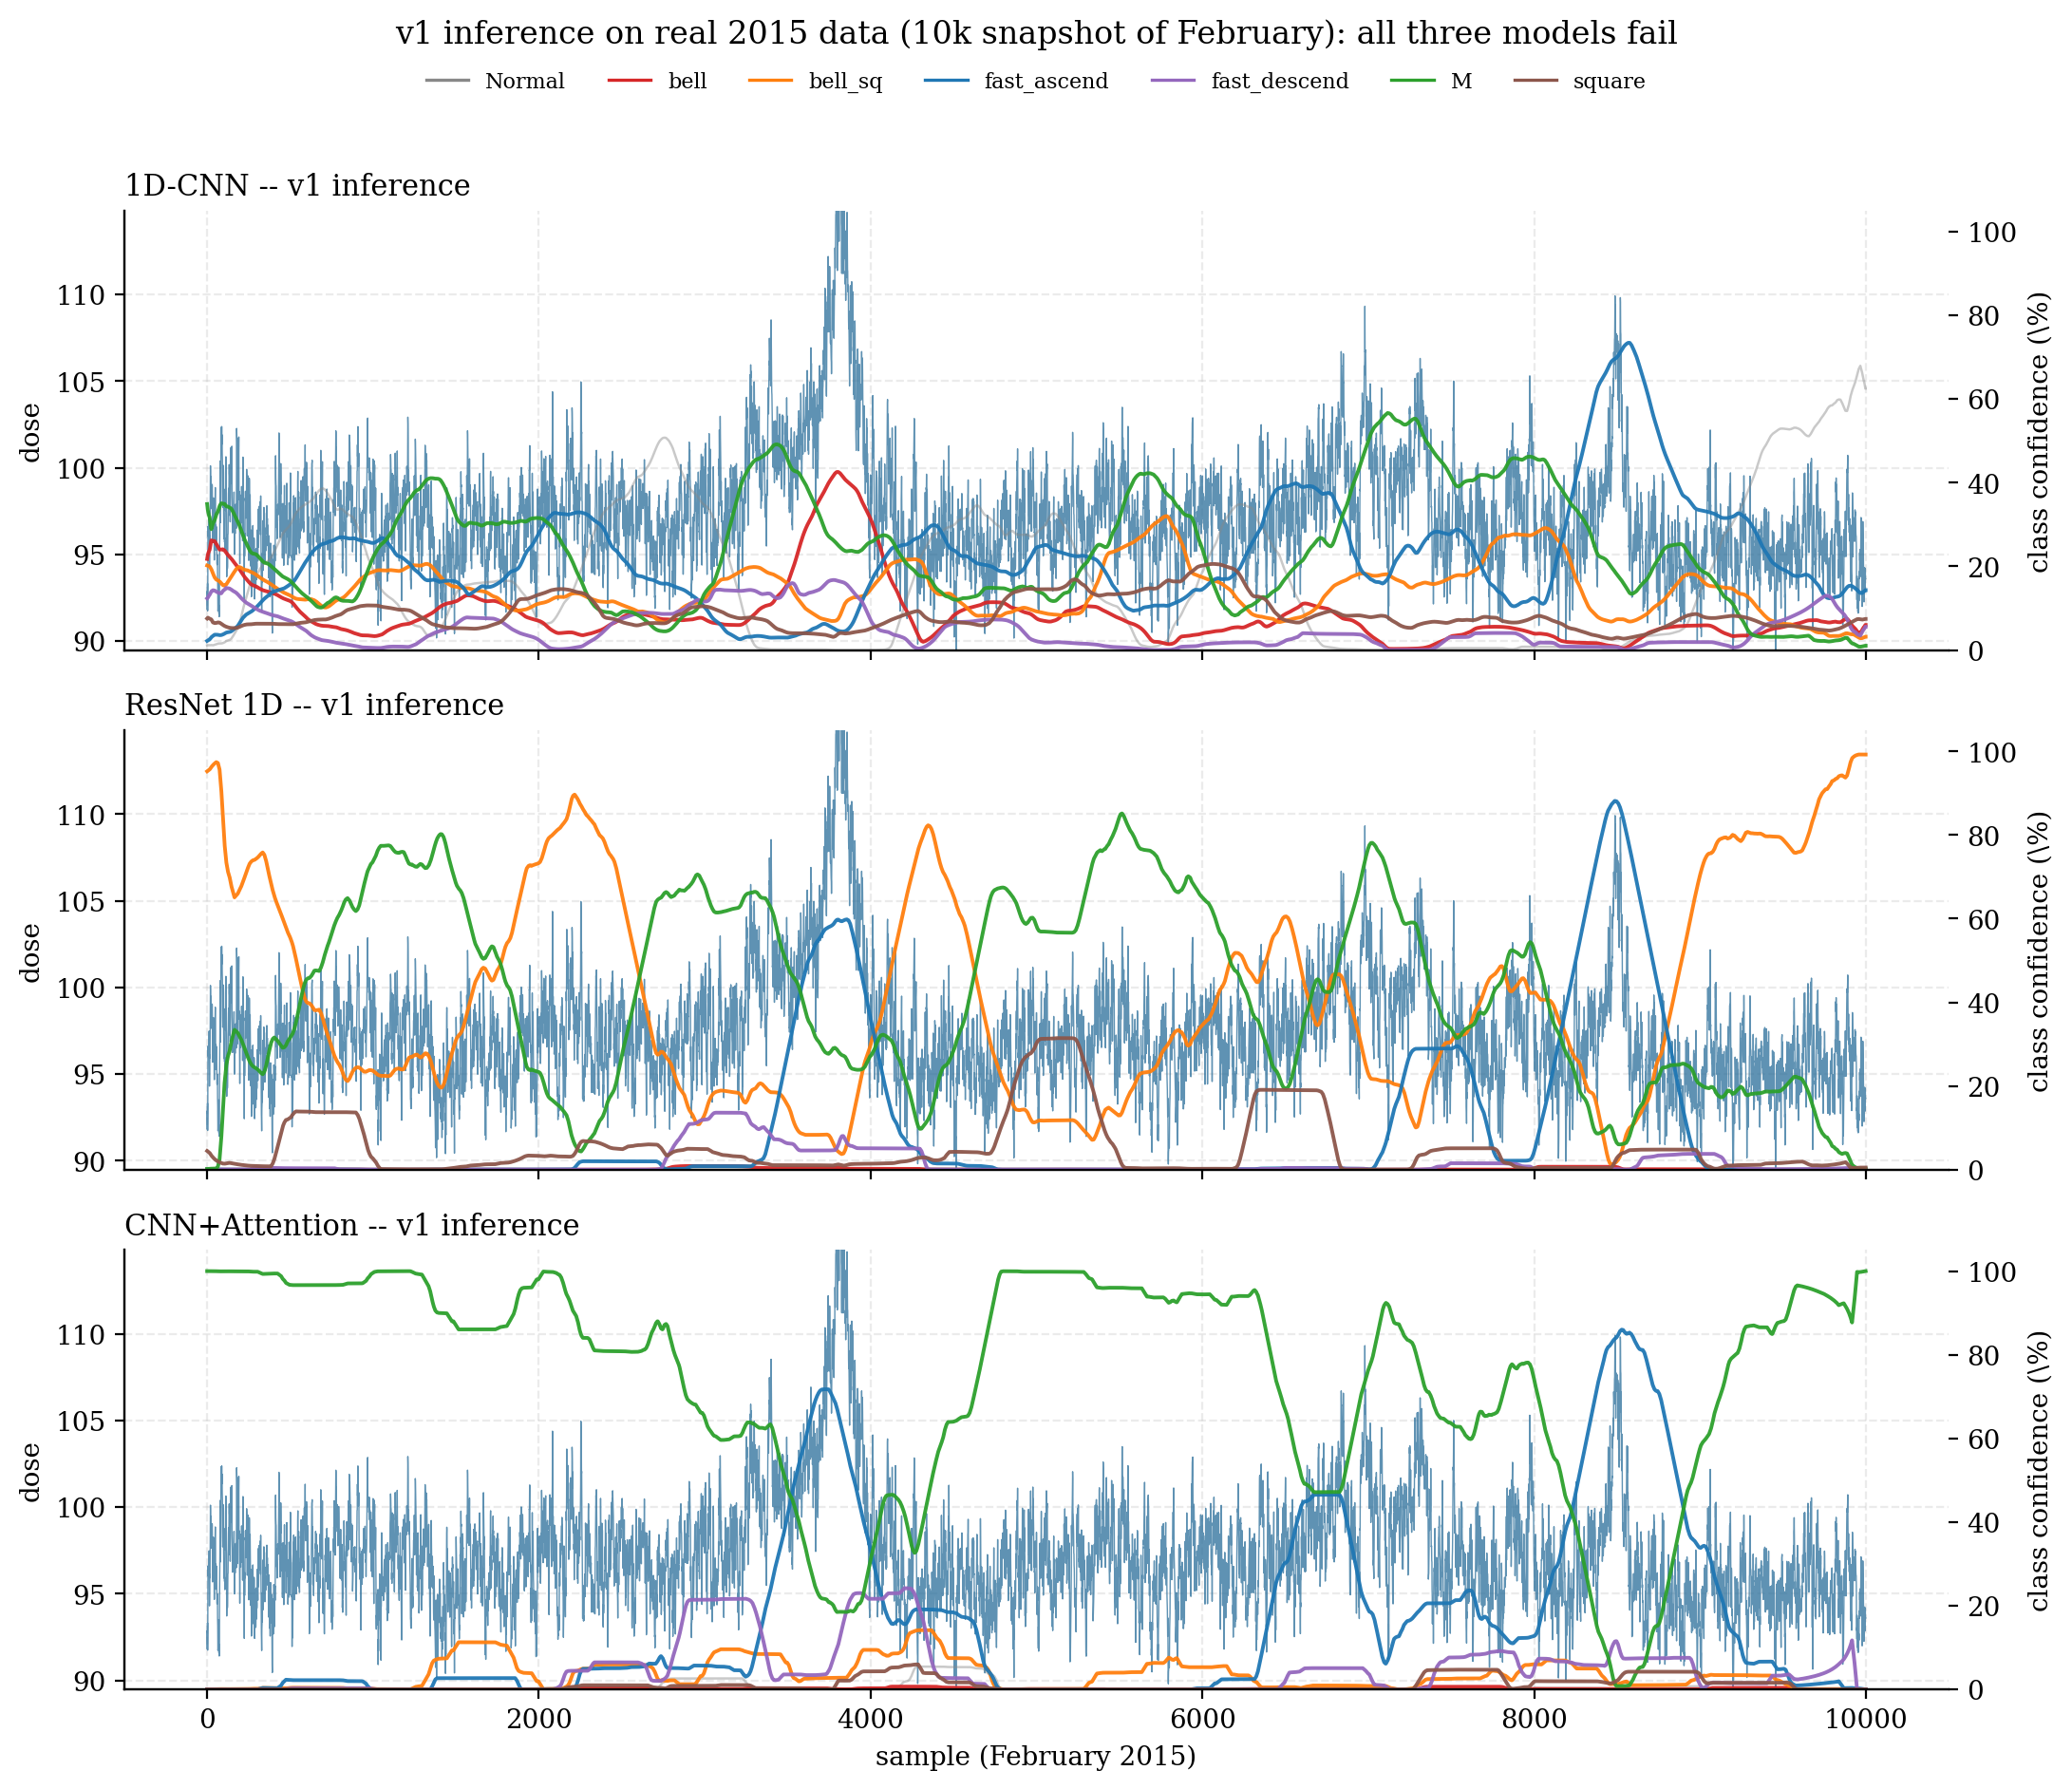
\includegraphics[width=\linewidth]{figures/v1_real_inference}
    \caption{v1 inference on the first $10\,000$ samples of February
    2015. Blue: raw gamma dose (left axis). Coloured lines: per-class
    confidence smoothed with a $30$-sample rolling mean (right axis,
    $0$--$100\%$). The grey curve is the \texttt{Normal Background}
    confidence; the other colours are the six anomaly classes.}
    \label{fig:v1-real-inference}
\end{figure}

\paragraph{1D-CNN --- high-frequency oscillating predictions.} Each
anomaly class takes its turn going up and down between $0\%$ and
$\sim 40\%$. The \texttt{Normal Background} probability sits in the
$50\%$--$70\%$ band but never crosses the operational threshold that
would make the system silent. A spike in \texttt{M} confidence around
sample $4\,000$ coincides with the visible bump in the raw signal ---
that part is encouraging --- but the same level of confidence is
reached elsewhere, in places where nothing is happening.

\paragraph{ResNet --- sustained false-positive plateaus.} The ResNet
does not oscillate; instead, it locks onto one anomaly class at a time
for long stretches. The orange \texttt{bell\_sq} confidence plateaus
near $100\%$ for thousands of samples; the green \texttt{M} confidence
does the same on the second half of the window. Every quiet region of
the signal is silently classified as one anomaly or another.

\paragraph{CNN+Attention --- degenerate collapse onto \texttt{M}.} The
hybrid model exhibits the most dramatic failure: the green \texttt{M}
confidence is pinned to $100\%$ for the entire $10\,000$-sample
snapshot. The signal could be flat at the global mean, and the model
would still declare \texttt{M} with full confidence.

The three failures share a single root cause --- a much larger
\emph{distribution shift} between training and deployment than the v1
noise model accounted for --- but they are amplified differently by
each architecture. We now look at the main mismatches.

\section{Five causes of the v1 failure}
\label{sec:v1-fail-causes}

\paragraph{Cause 1: training-vs-deployment class prior.} The v1
synthetic dataset has roughly $31\%$ \texttt{Normal} windows and
$\sim 11\%$ of each anomaly class. The real recordings have
$> 99\%$ \texttt{Normal} (only $17$ plausible events in
$4 \times 40\,000$ samples). The two priors are roughly
\emph{opposite}. On top of this, v1's class-weight vector
$\mathbf{w}_{\text{v1}}$ down-weights \texttt{Normal} by a factor
$\sim 2.7$ relative to the anomaly classes, which from a Bayesian
perspective is equivalent to multiplying the network's posterior on
the anomaly classes by another factor of $\sim 2.7$ at deployment.
The deployment posterior is therefore mis-calibrated by a factor of
roughly $200$.

\paragraph{Cause 2: anomaly-duration mismatch.} The v1 templates have
durations in $[200, 800]$ samples. The hand-labelled real events span
$32$ to $1\,014$ samples (\cref{sec:reanalysis-labels}), with several
events of $\sim 50$ samples that fall well outside the v1 range.

\paragraph{Cause 3: noise-texture mismatch.} The v1 background is IID
Gaussian. The real residual is autocorrelated with lag-1 ACF $\approx
0.86$ (\cref{chap:reanalysis}). A $512$-sample window therefore sees a
very different local texture in synthetic vs.\ real --- much
``rougher'' in v1 because the samples are independent, much smoother in
the real signal because of the AR(1) memory. The marginal histogram
of values inside the window is identical in both cases ($\sigma \approx
2.3$), so any model that looks only at the marginal sees no shift, but
a 1D convolutional layer extracting features from local patches of a
few samples sees a fundamentally different input.

\paragraph{Cause 4: side-effects of per-window centring.} The window
mean is subtracted before every forward pass (\cref{eq:window-norm}).
On the v1 synthetic test set this is harmless because the events
occupy a known fraction of the window. On a real long contamination
plateau that covers most of the window, the window mean is dragged up
by the event itself; after centring, the event has \emph{lost most of
its amplitude} and only its edges survive.

\paragraph{Cause 5: no ``background-but-not-Normal'' class.} A v1
window either contains a clean templated event or pure stationary
background. Real recordings contain a much richer family of
intermediate signals (a slow drift, an outlier sample, a brief sensor
wobble) that are neither a clean event nor pure stationary noise. With
no class to assign to those, and (because of cause 1) a bias towards
the anomaly classes, the network is forced into a wrong choice on
every quiet region.

\paragraph{Why the failure mode depends on the architecture.} The five
causes are shared; the failure mode is not.
\begin{itemize}[leftmargin=*, itemsep=0.2em]
    \item \textbf{1D-CNN with BatchNorm.} BatchNorm running statistics
    accumulated during training are wrong at deployment, so the
    normalised activations are wildly different from anything the
    network saw at training; the classifier head can no longer commit
    to a single class and oscillates.
    \item \textbf{ResNet with GroupNorm.} GroupNorm is per-window, so
    normalisation behaves identically at training and deployment ---
    the activations are valid, the features are stable --- but the
    classifier head is still mis-calibrated by the prior shift, so it
    coherently and confidently picks the wrong class.
    \item \textbf{CNN+Attention.} The attention layer aggregates the
    entire window into a single CLS token; when the window is
    out-of-distribution, the CLS aggregation converges to a single
    mode (the most ``textured'' class, \texttt{M}) regardless of the
    input.
\end{itemize}

\section{What to do about it}
\label{sec:v1-remediation}

The five causes translate into a concrete remediation list, which is
exactly what motivates the v2 generator of \cref{chap:v2gen}:

\begin{enumerate}[leftmargin=*, itemsep=0.2em]
    \item \textbf{Match the deployment prior.} Lower the synthetic
    anomaly density by an order of magnitude (cause 1).
    \item \textbf{Match the noise texture.} Replace the IID Gaussian
    residual by an AR(1) Gaussian fitted to the real data (cause 3).
    \item \textbf{Match the anomaly amplitude and duration ranges.}
    Drive both from the hand-labelled real events; in particular, drop
    the artificial duration floor at $200$ samples and extend the
    range down to $\sim 30$ (cause 2).
    \item \textbf{Drop the templates that do not occur in the real
    labels.} The \texttt{M}, \texttt{bell\_sq}, \texttt{square}
    templates have no counterpart in the hand labels and are exactly
    the classes the v1 networks collapsed onto on out-of-distribution
    input (cause 5).
    \item \textbf{Hand-label a small set of real events} to drive the
    above three calibrations (and to detect, after re-training, whether
    the corrections worked).
\end{enumerate}

Causes 1--3 are addressed by the v2 generator
(\cref{chap:reanalysis,chap:v2gen}). Cause 4 (per-window centring) is
not changed in v2 --- the empirical durations in the labels stay
shorter than $512$ samples on most events, so the per-window centring
remains a reasonable inductive bias. Cause 5 is partially addressed by
dropping the unused templates, but a dedicated ``unknown but not
\texttt{Normal}'' class is left for future work.

The next chapter walks through the re-analysis of the real background
that produces, in particular, the AR(1) noise model used in v2.
